\section{GP-MP Algorithm}
\label{sec:overall}

\subsection{Overall Algorithm}
\label{sec:schedule}

The trained denoiser provides the channel mean
$\mathbf F_k=\mathbf F_\theta(\mathbf R_k,v)$, while the variance
estimate $\widehat\tau_k=\widehat\tau_\theta(\mathbf R_k,v)$ is given by
\eqref{eq:derivative-trace}.
Averaging $\widehat\tau_k$ over devices and applying the positive lower
bound $\tau_{\min}$ gives $\tau^{\rm post}$.
The trained activity classifier provides $p_k$ through
\eqref{eq:activity-probability}.

Fig.~\ref{fig:learned-receiver} illustrates the generative-prior
message-passing (GP-MP) receiver, in which GPJD uses the trained
denoiser and activity classifier, while MFLE is derived analytically.

\begin{figure*}[!t]
\centering
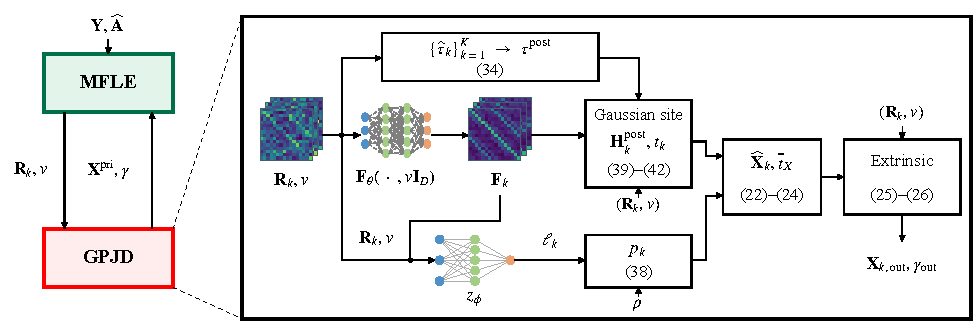
\includegraphics[width=0.92\textwidth]{learned_receiver.pdf}
\caption{Message exchange between MFLE and GPJD, with an expanded view of GPJD.
The denoising illustration follows \cite{cai2026}.}
\label{fig:learned-receiver}
\end{figure*}

The phases are either known or estimated once before MP and remain
fixed during the iterations. For initialization, $\widehat P_H$ is the
normalized training-channel power, computed by averaging
$\norm{\mathbf H}_F^2/D$ over the training channels.

Algorithm~\ref{alg:gp-mp-ccd} presents the pseudocode for GP-MP.

\begin{figure}[!t]
\centering
\begin{minipage}{\linewidth}
\small
\refstepcounter{algorithm}\label{alg:gp-mp-ccd}
\hrule\vspace{3pt}
\textbf{Algorithm \thealgorithm}\enspace GP-MP for JADCE\par
\vspace{3pt}\hrule\vspace{3pt}
\begin{algorithmic}[1]
 \Require $\mathbf Y$, $\{\mathbf p_{qk}\}$, available phases, $\rho$, trained
 $\mathbf f_\theta$ and $z_\phi$.
 \Ensure $\{s\widehat{\mathbf X}_k,s\mathbf H_k^{\rm post},p_k,\widehat\alpha_k\}_{k=1}^K$.
 \State Estimate $\widehat\sigma^2$; estimate any unknown phases once as described in
 Section~\ref{sec:phase-estimation}.
 \State Construct $\widehat{\mathbf A}$ using fixed phases; normalize $\mathbf Y$ and $\widehat\sigma^2$ as in Section~\ref{sec:frontend}.
 \State Compute the SVD of $\widehat{\mathbf A}$; draw one random sign vector
 per device and reuse it across iterations.
 \State Initialize $\mathbf X^{{\rm pri},(0)}\gets\mathbf0$,
 $\gamma^{(0)}\gets\rho\widehat P_H$.
 \State Initialize $\mathbf E_k\gets\mathbf0$, $\tau_k^{\rm ext}\gets1$,
 $\kappa^{(1)}\gets1$.
 \For{$i=1,\ldots,I_{\max}$}
  \Statex \hspace{\algorithmicindent}\textit{\% MFLE}
  \State Update $\mathbf R_{{\rm L},k}$ and $v_{\rm L}$ by
  \eqref{eq:linear-mean}--\eqref{eq:linear-extrinsic-mean}, using
  \eqref{eq:linear-fraction}--\eqref{eq:linear-svd-extrinsic}.
  \State $\mathbf R_k\gets\mathbf R_{{\rm L},k}$, $\bar v\gets v_{\rm L}$;
  apply \eqref{eq:input-damping}--\eqref{eq:input-variance-damping} for $i\geq2$.
  \State $v\gets\kappa^{(i)}\bar v$.
  \Statex \hspace{\algorithmicindent}\textit{\% GPJD}
  \State $\mathbf F_k\gets\mathbf F_\theta(\mathbf R_k,v)$.
  \State Compute $\widehat\tau_k$ and $p_k$ by \eqref{eq:derivative-trace}
  and \eqref{eq:activity-probability}.
  \State Average $\widehat\tau_k$ over $k$ to obtain $\tau^{\rm post}$.
  \State Apply the lower bound $\tau_{\min}$ to $\tau^{\rm post}$.
  \If{$\tau^{\rm post}<v$}
   \State Update $\mathbf E_k$ and $\tau_k^{\rm ext}$ by
   \eqref{eq:site-update}--\eqref{eq:site-mean}.
  \EndIf
  \State Update $\mathbf H_k^{\rm post}$ and $t_k$ by
  \eqref{eq:conditional-moments}--\eqref{eq:conditional-channel-mean}.
  \State Update $\widehat{\mathbf X}_k$ and $\overline t_X$ by
  \eqref{eq:mixture} and \eqref{eq:joint-average-variance}.
  \State Update $\kappa^{(i+1)}$ as in Section~\ref{sec:variance-update}.
  \State Compute $\mathbf X_{k,\rm out}$ and $\gamma_{\rm out}$ by
  \eqref{eq:nonlinear-extrinsic}--\eqref{eq:nonlinear-extrinsic-mean} with clipping.
  \State $\mathbf X_k^{{\rm pri},(i)}\gets\mathbf X_{k,\rm out}$,
  $\gamma^{(i)}\gets\gamma_{\rm out}$; apply
  \eqref{eq:output-damping}--\eqref{eq:output-variance-damping} for $i\geq2$.
  \State Update the stopping history.
  \If{the stopping conditions in Section~\ref{sec:stopping-criteria} hold}
   \State \textbf{break}
  \EndIf
 \EndFor
 \State $\widehat\alpha_k\gets\mathbf1\{p_k\geq1/2\}$.
 \State \Return $\{s\widehat{\mathbf X}_k,s\mathbf H_k^{\rm post},p_k,\widehat\alpha_k\}_{k=1}^K$.
\end{algorithmic}
\vspace{3pt}\hrule
\end{minipage}
\end{figure}

\subsection{Parameter Estimation and Numerical Implementation}
\label{sec:frontend}
\label{sec:phase-estimation}
\label{sec:variance-update}
\label{sec:damping}

For noise estimation, the Wax--Kailath minimum description length
(MDL) criterion \cite{wax1985,nadakuditi2008} is used to estimate the
signal covariance rank $\widehat r_{\rm s}$ based on the eigenvalues
$\lambda_1\geq\cdots\geq\lambda_M$ of the sample covariance matrix.
Let $\mathbf y_{qr}$ denote column $r$ of $\mathbf Y_q$ and
$N_{\rm s}=QN>M\geq2$. The sample covariance and noise estimate are
\begin{align}
 \widehat{\mathbf R}_y&=\frac1{N_{\rm s}}\sum_{q,r}
 \mathbf y_{qr}\mathbf y_{qr}^{\mathsf H},
 \label{eq:sample-spatial-covariance}\\
 \widehat\sigma^2&=\frac{\sum_{i=\widehat r_{\rm s}+1}^{M}\lambda_i}
 {M-\widehat r_{\rm s}}.
 \label{eq:noise-estimation}
\end{align}
This estimate assumes a low-rank signal covariance and is held fixed
during MP.

For phase estimation, the observations are stacked into the matrix
$\mathbf Y_{\rm s}=[\mathbf Y_0,\ldots,\mathbf Y_{Q-1}]^{\mathsf T}
\in\mathbb C^{QN\times M}$.
The dominant line-of-sight component of the default NTN-TDL-D
channel motivates a single-path approximation of each device's
channel for estimating its common Doppler shift. Absorbing the common scalar
phase into the path gain gives
\begin{equation}
 [\mathbf h_k^{\rm p}(d,\nu)]_{qN+r}
 =e^{\mathrm j2\pi\nu qT_{\rm frame}}
 [\mathbf G_0(d,\nu)\mathbf p_{qk}]_r,
 \label{eq:phase-atom}
\end{equation}
where $\mathbf G_0(d,\nu)=e^{-\mathrm j2\pi c_1d^2}\mathbf G(d,\nu;0)$.

With $\mathbf h_k^{\rm p}=\mathbf h_k^{\rm p}(d_k,\nu_k)$, the
observations can be expressed as
$\mathbf Y_{\rm s}\approx\sum_k\mathbf h_k^{\rm p}\mathbf b_k^{\mathsf T}
+\mathbf W_{\rm s}$.
This observation model is complemented by independent Gaussian priors
over the gains, $\mathbf b_k\sim\CN(\mathbf0,\gamma_k\I_M)$,
$\gamma_k\geq0$.
Phase estimation is formulated as the minimization of the negative log
marginal likelihood \cite{tipping2003}, obtained by integrating out
the gains:
\begin{align}
 \mathbf S&=\widehat\sigma^2\I_{QN}
 +\sum_k\gamma_k\mathbf h_k^{\rm p}\mathbf h_k^{{\rm p},\mathsf H},
 \label{eq:phase-covariance}\\
 \mathcal L&=\log\det\mathbf S+
 \frac1M\tr(\mathbf Y_{\rm s}^{\mathsf H}\mathbf S^{-1}\mathbf Y_{\rm s}).
 \label{eq:phase-objective}
\end{align}
The objective $\mathcal L$ is minimized by coordinate updates, with
each $\gamma_k$ solved for analytically and $(d_k,\nu_k)$ refined
using L-BFGS-B
\cite{zhu1997}.

The estimated Doppler determines $\widehat\beta_k$ and
$\widehat{\mathbf A}$ through
\eqref{eq:twc-frame-channel}--\eqref{eq:effective-pilot}.

To match the scale used for denoiser training, the channel and
observation quantities $(\mathbf H_k,\mathbf X_k,\mathbf Y,\mathbf W)$
are divided by the root mean square $s$ of the training-channel
entries, and the noise variance is divided by $s^2$.
The same symbols denote the normalized quantities.

In each iteration, the mean and variance updates are damped using a
linear combination of the current update and the previous damped
message \cite{rangan2019}.
With damping factor $\eta\in(0,1]$, the input messages to GPJD for
$i\geq2$ are
\begin{align}
 \mathbf R_k^{(i)}&=(1-\eta)\mathbf R_k^{(i-1)}+\eta \mathbf R_{{\rm L},k}^{(i)},
 \label{eq:input-damping}\\
 \bar v^{(i)}&=(1-\eta)\bar v^{(i-1)}+\eta v_{\rm L}^{(i)}.
 \label{eq:input-variance-damping}
\end{align}
At iteration $i$, GPJD uses $v^{(i)}=\kappa^{(i)}\bar v^{(i)}$.
After joint denoising, the update of the input variance follows from
minimizing the expected Gaussian negative log likelihood, with the current
approximate posterior held fixed \cite{vila2013}.
Setting the derivative with respect to the variance to zero yields
\begin{equation}
 v_{\rm tar}=\frac{1}{KD}\sum_{k=1}^K
 \norm{\mathbf R_k-\widehat{\mathbf X}_k}_F^2+\overline t_X.
 \label{eq:query-variance-target}
\end{equation}
The next scaling factor $\kappa^{(i+1)}$ is obtained by averaging
$\kappa^{(i)}$ and $v_{\rm tar}^{(i)}/\bar v^{(i)}$ with weights
$1-\eta$ and $\eta$, respectively.

The input to MFLE is damped in a similar manner.
In the feedback updates
\eqref{eq:nonlinear-extrinsic}--\eqref{eq:nonlinear-extrinsic-mean},
$b=\overline t_X/v$ is clipped to $[\varepsilon,1-\varepsilon]$,
where $0<\varepsilon<1/2$.
With the same damping factor, the feedback messages for $i\geq2$ are
\begin{align}
 \mathbf X_k^{{\rm pri},(i)}
 &=(1-\eta)\mathbf X_k^{{\rm pri},(i-1)}+\eta \mathbf X_{k,\rm out}^{(i)},
 \label{eq:output-damping}\\
 \gamma^{(i)}
 &=(1-\eta)\gamma^{(i-1)}+\eta\gamma_{\rm out}^{(i)}.
 \label{eq:output-variance-damping}
\end{align}

\subsection{Computational Complexity Analysis}
\label{sec:complexity}

With precomputed chirp factors, $L$ AFDM frames require at most
$LC_{\rm FFT}(N)+2LN$ complex multiplications
\cite{bemani2022}, where $C_{\rm FFT}(n)$ is the cost of an
$n$-point fast Fourier transform (FFT) or inverse FFT. For the same $LN$ useful symbols,
rectangular-pulse OTFS without transmit windowing requires
$NC_{\rm FFT}(L)$ after cancelling the consecutive discrete Fourier transform (DFT)
and inverse DFT operations
\cite{zou2021otfs}.

The computational complexity of the receiver is primarily determined
by the operations in MFLE and GPJD, together with parameter estimation.
With fixed phases and $Q\leq KN$, MFLE can be implemented using the
singular value decomposition (SVD),
$\widehat{\mathbf A}=\mathbf U\diag(s_1,\ldots,s_Q)\mathbf V^{\mathsf H}$,
which is reused across iterations. Here $s_a$ are the singular values,
and the scalar updates in
\eqref{eq:linear-variance}--\eqref{eq:linear-extrinsic} can be written as
\begin{align}
 f_{\rm L}&=\frac{1}{KN}\sum_{a=1}^{Q}
 \frac{\gamma s_a^2}{\widehat\sigma^2+\gamma s_a^2},
 \label{eq:linear-fraction}\\
 t_{\rm L}&=\gamma(1-f_{\rm L}),
 \label{eq:linear-svd-variance}\\
 v_{\rm L}&=\frac{t_{\rm L}}{f_{\rm L}}.
 \label{eq:linear-svd-extrinsic}
\end{align}
Here $\mathbf R_{\rm L}=\mathbf X^{\rm pri} +(\mathbf X_{\rm L}-\mathbf
X^{\rm pri})/f_{\rm L}$.

For each block, the SVD and noise-variance estimation require
$O(KNQ^2)$ and $O(QNM^2+M^3)$ operations, respectively.
The phase-estimation cost is denoted by $C_{\rm phase}$, with
$C_{\rm phase}=0$ for known phases.

For each iteration, the MFLE transformations involve $O(QKMN^2)$
operations, while the spatial covariance operations and matrix
factorizations require $O(KM^2N^2)$ and $O(M^3)$ operations,
respectively. The per-device costs of a forward pass through the
denoiser and classifier are denoted by $C_\theta$ and $C_\phi$,
respectively. Each GPJD update evaluates the denoiser $1+2L_z$ times
and the classifier once per device. Consequently, these forward
passes require $K[(1+2L_z)C_\theta+C_\phi]$ operations.

Overall, the online complexity for $I$ iterations is
$O(C_{\rm phase}+QNM^2+M^3+KNQ^2+I C_{\rm iter})$, where
$C_{\rm iter}$ denotes the total per-iteration cost.
The pilot matrix, SVD factors, channel messages, and spatial
covariances require $O(QKN+KMN^2+KM^2)$ memory.
